%%%%%%%%%%%%%%%%%%%% author.tex %%%%%%%%%%%%%%%%%%%%%%%%%%%%%%%%%%%
%
% sample root file for your "contribution" to a contributed volume
%
% Use this file as a template for your own input.
%
%%%%%%%%%%%%%%%% Springer %%%%%%%%%%%%%%%%%%%%%%%%%%%%%%%%%%


% RECOMMENDED %%%%%%%%%%%%%%%%%%%%%%%%%%%%%%%%%%%%%%%%%%%%%%%%%%%
\documentclass[graybox]{svmult}

% choose options for [] as required from the list
% in the Reference Guide

\usepackage{mathptmx}       % selects Times Roman as basic font
\usepackage{helvet}         % selects Helvetica as sans-serif font
\usepackage{courier}        % selects Courier as typewriter font
\usepackage{type1cm}        % activate if the above 3 fonts are
                            % not available on your system
%
\usepackage{makeidx}         % allows index generation
\usepackage{graphicx}        % standard LaTeX graphics tool
                             % when including figure files
\usepackage{multicol}        % used for the two-column index
\usepackage[bottom]{footmisc}% places footnotes at page bottom

% see the list of further useful packages
% in the Reference Guide

\usepackage[hidelinks]{hyperref}


\makeindex             % used for the subject index
                       % please use the style svind.ist with
                       % your makeindex program


%----    Revision command    -----%
\definecolor{OliveGreen}{rgb}{0,0.6,0}
\definecolor{amber}{rgb}{1.0, 0.49, 0.0}
\newcommand{\todo}[1]{(\textcolor{red}{To do: #1})}
\newcommand{\claudio}[1]{(\textcolor{red}{Claudio: #1})}
\newcommand{\altoe}[1]{(\textcolor{blue}{Altoè: #1})}
\newcommand{\pastore}[1]{(\textcolor{OliveGreen}{Pastore: #1})}
\newcommand{\enrico}[1]{(\textcolor{amber}{Enrico: #1})}


%%%%%%%%%%%%%%%%%%%%%%%%%%%%%%%%%%%%%%%%%%%%%%%%%%%%%%%%%%%%%%%%%%%%%%%%%%%%%%%%%%%%%%%%%

\begin{document}

\title*{Incorporating Expert Knowledge in Structural Equation Models: Applications in Psychological Research}
\titlerunning{Incorporating Expert Knowledge in Structural Equation Models}
\subtitle{\emph{Integrare il Parere degli Esperti con i Modelli di Equazioni Strutturali: Applicazioni nella Ricerca Psicologica}}
\author{Gianmarco Alto\`e, Claudio Zandonella Callegher,  Enrico Toffalini and Massimiliano Pastore}
% Use \authorrunning{Short Title} for an abbreviated version of
% your contribution title if the original one is too long
\authorrunning{G. Alto\`e, C. Zandonella Callegher,  E. Toffalini and M. Pastore}
\institute{
Gianmarco Alto\`e \at Department of Developmental Psychology and Socialisation, University of Padova \\ \email{gianmarco.altoe@unipd.it}
\and Claudio Zandonella Callegher \at Department of Developmental Psychology and Socialisation, University of Padova \\ \email{claudio.zandonellacallegher@phd.unipd.it}
\and Enrico Toffalini \at Department of General
Psychology, University of Padova \\ \email{enrico.toffalini@yahoo.it}
\and Massimiliano Pastore \at Department of Developmental Psychology and Socialisation, University of Padova  \\
 \email{massimiliano.pastore@unipd.it}
}
%
% Use the package "url.sty" to avoid
% problems with special characters
% used in your e-mail or web address
%
\maketitle

\abstract{Structural Equation Modeling (SEM) is used in psychology to model  complex structures of data. However,  sample sizes often cannot be as large as ideal for SEM, leading to a problem of insufficient power. Bayesian estimation with informed priors can be beneficial in this context. Our simulation study examines this issue over a real case of a mediation model. Parameter recovery, power and coverage were considered. The advantage of a Bayesian approach was evident for the smallest effects. The correct formalization of the theoretical expectations is crucial, and it allows for increased collaboration among researchers in Psychology and Statistics.
}

% Structural Equation Modeling (SEM) is useful in psychological research, where complex structures of data must be modelled considering several sources of variability. Sample sizes in Psychology cannot be as large as ideal for SEM in most cases, and real effect sizes are generally small, leading to a widespread problem of insufficient power. Bayesian estimation with informed priors can be beneficial in this context. Our simulation study examines this issue over a real case of a mediation model. Parameter recovery, power and coverage were considered. The advantage of a Bayesian approach was evident for the smallest effects. Expert knowledge elicitation, i.e., the correct formalization of the theoretical expectations, is crucial and it allows for increased collaboration among researchers in Psychology and Statistics.
\abstract{\emph{I Modelli di Equazioni Strutturali (SEM) sono spesso utilizzati in psicologia. Tuttavia, campioni limitati portano ad un problema di insufficiente potenza. Il nostro studio di simulazione esamina i vantaggi dell'approccio bayesiano con prior informative nel caso di un modello di mediazione. Sono state considerate la stima dei parametri, gli intervalli di confidenza e la potenza. Il vantaggio dell'approccio Bayesiano è risultato evidente per gli effetti minori. La formalizzazione delle aspettative teoriche è cruciale e favorisce una fruttuosa collaborazione tra i ricercatori.
}}

% I Modelli di Equazioni Strutturali (SEM) sono utilizzati in psicologia per indagare fenomeni complessi. In psicologia le dimensioni degli effetti sono generalmente piccole e i campioni di studio non ideali per l'approccio SEM, portando a un problema di insufficiente potenza. La stima bayesiana con prior informative può essere utile in questo contesto. Il nostro studio di simulazione esamina questo problema nel caso reale di un modello di mediazione. Sono state considerate la stima dei parametri, gli intervalli di confidenza e la potenza. Il vantaggio dell'approccio Bayesiano è risultato evidente per gli effetti più piccoli. La formalizzazione della conoscenza degli esperti e delle aspettative teoriche è cruciale soprattutto nell'ottica di favorire una fruttuosa collaborazione tra ricercatori in Psicologia e Statistica.



\keywords{Expert elicitation, Informative Priors, Structural Equation Models (SEM), Small sample sizes, Psychological research}

\section{Introduction}
\label{sec:1}



\emph{Structural Equation Modeling} (SEM) encompasses  a range of multivariate statistical techniques. SEMs are composed of two parts: a \emph{measurement model} and a \emph{structural model} (see Fig.~\ref{fig:example_sem}).   The measurement model defines unobserved constructs (\emph{latent variables}, circles in Fig.~\ref{fig:example_sem}) according to a set of measured outcomes (\emph{observed variables}, squaes in Fig.~\ref{fig:example_sem}), whereas the structural model describes the relationships between latent variables.
% \emph{Structural Equation Modeling} (SEM) encompasses  a range of multivariate statistical techniques as, for example, confirmatory factor analysis, path analysis, or latent growth modeling. Generally, SEMs are composed of two parts: a \emph{measurement model} and a \emph{structural model} (see Fig.~\ref{fig:example_sem}).   The measurement model defines unobserved constructs (\emph{latent variables}, represented in Fig.~\ref{fig:example_sem} as circles) according to a set of measured outcomes (\emph{observed variables}, represented in Fig.~\ref{fig:example_sem} as squares), whereas the structural model describes the relationships between latent variables.
%zIn SEM, parameters are estimated by minimizing a discrepancy function between the sample covariance matrix and the covariance matrix implied by the model.
\begin{figure}[b]
	\sidecaption
	\label{fig:example_sem}
	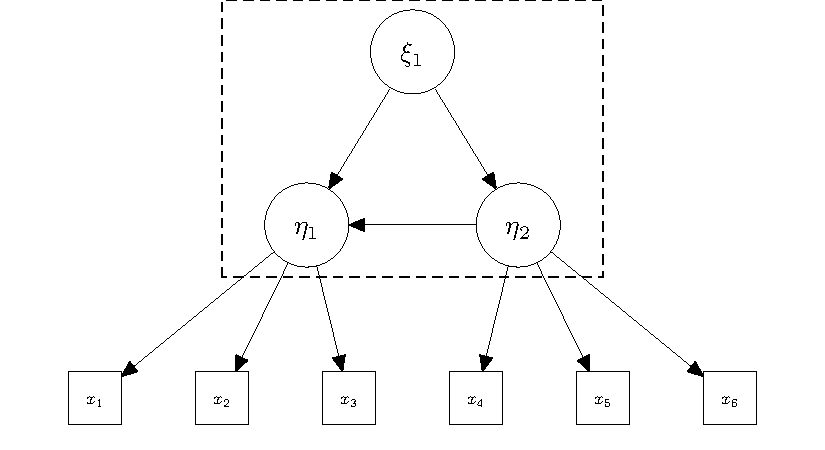
\includegraphics[width = .45\textwidth]{figure/Plot_SEM}
	\caption{A structural equation model. Within the dashed box is the structural model, outside is the measurement model. Circles for latent variables; rectangles for observed variables.}
\end{figure}
% Considering the covariance structure (instead of modeling all the observed data) allows to model complex relations between variables taking into account also the  measurement error.
% Given their great flexibility, SEMs are widely used in psychology for various purposes such as validating psychological tests and questionnaires or evaluating hypotheses and theoretical models that involve complex relations between different latent psychological constructs.
SEMs are widely used in psychology to model complex relations between different latent psychological constructs. However, as the complexity of the model increases, more data are required to obtain accurate parameter estimates and model fit statistics \cite{wolfSampleSizeRequirements2013}.
%Recent concerns about the replicability of psychological results have raised awareness on the importance of properly define an adequate sample size \cite{ioannidisWhyMostPublished2005, opensciencecollaborationEstimatingReproducibilityPsychological2015}.
% Nevertheless, in many research settings, the number of participants may be limited due to financial restriction, strict inclusion criteria, or clinical samples. In the case of small sample sizes, appropriate statistical techniques are required to enhance the reliability of the results.
Nevertheless, in many research settings, the number of participants may be limited and appropriate statistical techniques are required to enhance the reliability of the results.

% Often in the literature, the Bayesian approach is suggested over frequentist estimation when limited data are available \cite{mcneishUsingBayesianMethods2016a}.  In the context of small sample, the inclusion of prior information can help in the parameter estimation, but researchers have to carefully consider priors choice, as estimates are highly sensitive to the prior specification (or misspecification).
%The use of Bayesian statistical approach is increasing and availability of softwares, such as R-package \texttt{blavaan} \cite{merkleBlavaanBayesianStructural2018},  provide researchers with flexible tools for estimating even Bayesian structural equation models.
Often in the literature, the Bayesian approach is suggested over frequentist estimation when limited data are available \cite{mcneishUsingBayesianMethods2016a}.  The inclusion of prior information can help in the parameter estimation, but researchers have to carefully consider priors choice.
However, most of the studies rely on default software prior settings. A recent review, underlined that the use of diffuse default priors can result in severely biased estimates, and this bias can be decreased only by incorporating informative priors \cite{smidBayesianFrequentistEstimation2020}.
% However, most of the studies are unlikely to carefully consider priors choices, and often they rely on default software prior settings. A recent review, considering the performance of Bayesian estimation for structural equation models with small sample sizes, underlined that the use of diffuse default priors can result in severely biased estimates, and this bias can be decreased only by incorporating informative priors \cite{smidBayesianFrequentistEstimation2020}.
%Thus, authors warn against the use of \emph{naive prior} (i.e., diffuse default priors) when samples are small, and encourage researchers to incorporate \emph{thoughtful priors} (i.e., informative priors).

% Informative priors allow researchers to include in the analysis relevant knowledge in the field, such as previous studies results, meta-analyses or expert opinions.
% Informative priors allow researchers to include in the analysis relevant knowledge in the field. Priors choice should be clearly discussed and researchers are required to evaluate the generalizability of external information to the specific characteristics of their study. Researchers could also consider to include opinions of experts. On the base of their experience in the field, experts can evaluate relevant information and help researchers in the definition of a plausible range of values and priors choice.
%When the number of available studies is limited or their quality is judged not adequate, relying only on previous results in the literature could be misleading. In these cases, researchers could consider to include opinions of experts as well. On the base of their experience in the field, experts can evaluate relevant information and help researchers in the definition of a plausible range of values and priors choice.
Informative priors allow researchers to include in the analysis relevant knowledge in the field. Researchers could also consider to include opinions of experts. On the base of their experience in the field, experts can evaluate relevant information and help researchers in the definition of a plausible range of values and priors choice. \emph{Elicitation} is a structured procedure that allows experts to express their knowledge and uncertainty about quantities of interest in the form of probability distributions \cite{ohaganExpertKnowledgeElicitation2019,ohaganUncertainJudgementsEliciting2006}. Elicitation can be used to define priors according to  experts' judgement.

%The aim is to make a subjective judgement as much objective as possible by limiting potential sources of bias, forcing the experts to carefully reason about the answer, and by documenting and transparently reporting the whole procedure \cite{ohaganUncertainJudgementsEliciting2006}.

% Different elicitation methods have been proposed in the literature such as the \emph{Cooke protocol} \cite{cookeExpertsUncertaintyOpinion1991}, the \emph{Delphi method} \cite{roweDelphiTechniqueForecasting1999} or the \emph{SHELF protocol} \cite{oakleySHELFSheffieldElicitation2016}. The common aim of these methods is to make a subjective judgement as much objective as possible by limiting potential sources of bias, forcing the experts to carefully reason about the answer, and by documenting and transparently reporting the whole procedure.

% Elicitation methods differ in the solutions adopted and in the emphasis given to the different aspects of the elicitation. Researchers willing to conduct an elicitation process should evaluate the pros and cons of each method considering their own needs and constraints such as availability of experts, the possibility to group experts together, number of quantities to elicit or financial and time constraints.

% The remainder of this article is structured as follows. In Sec.~\ref{sec:simulation}, we present a simulation study to evaluate the influence of different prior specifications in the case of structural equation models with small sample size, considering an applied example of a mediation model in psychology. Although one of the major strengths of SEMs is to explicitly take measurement error associated with the latent variables into account, for the sake of simplicity (but without losing generalizability) we present a case in which the measurement model is not considered. It should also be noted that, following common procedures, all variables were standardized (i.e., mean = 0 and a standard deviation = 1) before fitting all models. In Sec.~\ref{sec:dicussion}, we discuss the obtained results highlighting limits and future developments of using expert knowledge with structural equation models in the case of  small sample sizes.


The remainder of this article is structured as follows. In Sec.~\ref{sec:simulation}, we present a simulation study to evaluate the influence of different prior specifications in the case of SEM with small sample size. For the sake of simplicity (but without losing generalizability) we present a mediation model in which the measurement model is not considered. Following common procedures, all variables were standardized (i.e., mean = 0 and a standard deviation = 1) before fitting all models. In Sec.~\ref{sec:dicussion}, we discuss the obtained results.


% \section{Expert knowledge elicitation}
% \label{sec:expert_elicitation}

% \emph{Elicitation} is a structured procedure that allows experts to express their knowledge and uncertainty about quantities of interest in the form of probability distributions \cite{ohaganExpertKnowledgeElicitation2019}. Elicitation can be used to define priors according to  experts' judgement.
%
% Different elicitation methods have been proposed in the literature such as the \emph{Cooke protocol} \cite{cookeExpertsUncertaintyOpinion1991}, the \emph{Delphi method} \cite{roweDelphiTechniqueForecasting1999} or the \emph{SHELF protocol} \cite{oakleySHELFSheffieldElicitation2016}. The common aim of these methods is to make a subjective judgement as much objective as possible by limiting potential sources of bias, forcing the experts to carefully reason about the answer, and by documenting and transparently reporting all the procedure.

% In general, elicitation is composed of three phases \cite{ohaganUncertainJudgementsEliciting2006}:
% \begin{enumerate}
% 	\item{\emph{Preparation and training} - experts are informed about  the aim of the elicitation and the parameters and quantities to elicit are clearly defined. All the relevant information about the topic of interest is collected and made available to experts. Next, experts are trained to make probabilistic judgements and they are familiarize with the elicitation process in a practice example to avoid misunderstandings. }
% 	\item{\emph{Individual judgements elicitation} - experts express their own judgement for each parameter or quantity of interest according to the elicitation technique they were trained before. Two of the main elicitation technique are the \emph{quartile method} and the \emph{roulette method}. In the former, experts provide values for the medians  and the quartile of the distribution according to their expectation. In the latter, the range of plausible values is divided into different intervals and the experts can place a given number of tokens to allocate probabilities according to  their expectation.}
% 	\item{\emph{Aggregation of individual judgements} - the individual judgements of the different experts are aggregate to obtain a unique final distribution. The two principal approaches are \emph{mathematical  aggregation}, where distributions are combined mathematically according to a pooling rule, and \emph{behavioral aggregation}, where experts are required to discuss together their opinions and reach a consensus judgement from which the aggregate distribution is obtained.}
% \end{enumerate}

% Elicitation methods differ in the solutions adopted during each phase and in the emphasis given to the different aspects of the elicitation.
% %For example, in the Cooke protocol experts are not required to meet each other. Experts return a form with their individual answer and mathematical aggregation is used to summarize the results. In the SHELF protocol, instead, much more emphasis is given to the collaboration between experts. After the  individual judgments, experts discuss and share their opinions to then reach a common final answer.
% Researchers willing to conduct an elicitation process should evaluate the pros and cons of each methods considering their own needs and constraints such as availability of experts, the possibility to group experts together, number of quantities to elicit or financial and time constraints.

\section{Simulation}
\label{sec:simulation}

% To evaluate the influence of different prior specifications in the case of structural equation models with small sample size, we considered a mediation model from \cite{sellaPersonalityTraitsSleep2020}  presented in Fig.~\ref{fig:example_model}.
We considered a mediation model from \cite{sellaPersonalityTraitsSleep2020}  presented in Fig.~\ref{fig:example_model}.
\begin{figure}[t]
	\sidecaption
	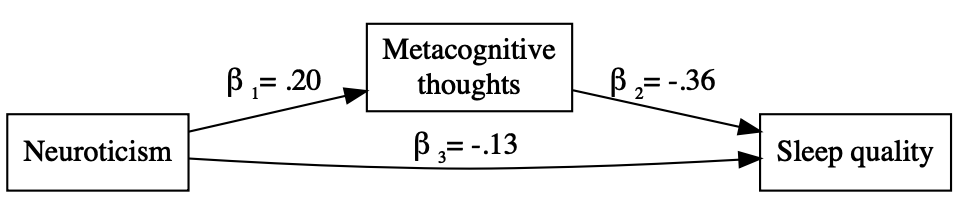
\includegraphics[width = .64\textwidth]{figure/Plot_example_model}
	\caption{Mediation model from \cite{sellaPersonalityTraitsSleep2020}. The relation between Neuroticism and sleep quality is mediated by metacognitive thoughts.}
	\label{fig:example_model}
\end{figure}
% The study evaluated the relationship between participants' self-reported sleep quality, personality characteristics, and negative beliefs about sleeping problems. In particular, the study found that the association between participants' tendency to experience distress and become anxious (\emph{Neuroticism}) and self-reported sleep quality (\emph{Sleep quality}) is small ($\beta_3=-.13$).  A stronger association is given  by the mediation role of the participants tendency to have negative thoughts about sleeping difficulties (\emph{Metacognitive thoughts}). In other words, people with higher levels of distress and anxiety tend to have dysfunctional beliefs and attitudes about sleep ($\beta_1=.20$) that, in turns, induce them to perceive and report a worse-quality sleep ($\beta_2=-.36$).
The study evaluated the relationship between participants' self-reported sleep quality (\emph{Sleep quality}), participants' tendency to become anxious (\emph{Neuroticism}), and negative beliefs about sleeping problems (\emph{Metacognitive thoughts}). In particular, the association between \emph{Neuroticism} and \emph{Sleep quality} ($\beta_3=-.13$) is mediated by \emph{Metacognitive thoughts}. In other words, people with higher levels of distress and anxiety tend to have dysfunctional beliefs and attitudes about sleep ($\beta_1=.20$) that, in turns, induce them to perceive and report a worse-quality sleep ($\beta_2=-.36$).


\subsection{Simulation details}

% The simulation was carried in \texttt{R} version 3.6.2 \cite{rcoreteamLanguageEnvironmentStatistical2018} using R-packages \texttt{lavaan} \cite{rosseelLavaanPackageStructural2012} and \texttt{blavaan} \cite{merkleBlavaanBayesianStructural2018}. In the simulation, we  considered as parameters of interest the regression coefficients ($\beta_1,\ \beta_2,\ \beta_3$) of the model presented above. We compared the performance of Maximum Likelihood (ML) estimation and Bayesian estimation under four different sample size conditions (i.e., 20, 50, 100, 500).

The simulation was carried in \texttt{R} version 3.6.2 \cite{rcoreteamLanguageEnvironmentStatistical2018} using R-packages \texttt{lavaan} \cite{rosseelLavaanPackageStructural2012} and \texttt{blavaan} \cite{merkleBlavaanBayesianStructural2018}. In the simulation, we  considered as parameters of interest the regression coefficients ($\beta_1,\ \beta_2,\ \beta_3$). We compared the performance of Maximum Likelihood (ML) estimation and Bayesian estimation under four different sample size conditions (i.e., 20, 50, 100, 500).

%In the current case, sample sizes below 100 can be considered small, whereas 500 is a more appropriate sample size and is considered as a reference benchmark.

Three different prior distribution specifications were used (see Fig.~\ref{fig:prior}):
\begin{enumerate}
	% \item{\textit{Default prior} -  in \texttt{blavaan}, default priors for regression coefficients are $N(0,10)$}. These priors are diffused over a wide range of values (95\% CI\ [-19.6;\ 19.6]) and are intended to be non-informative.
% 	\item{\textit{Reasonable prior} - the priors are $\beta_1\sim N(.20,\ .50)$, and  $\beta_{2;3}\sim N(-.20,\ .50)$, that correspond, respectively, to a 95\% CI of  [-.78;\ 1.18] and  [-1.18; .78]. These priors are moderately informative, they are intended to exclude excessively large values that are not reasonable within psychology research. Moreover, the mean of each prior distribution is slightly moved above or below zero to reflect the direction of the main results in the literature for each relation.}
%  	\item{\textit{Experts prior} - the priors are $\beta_1\sim N(.20,\ .20)$,  $\beta_{2}\sim N(-.40,\ .20)$}, and $\beta_3\sim N(-.20,\ .20)$, that correspond, respectively, to a 95\% CI of  [-0.19;\ .59], [-0.79;\ .01], and  [-.59; .19]. These priors are intended to be highly informative, they are intended to represent experts' judgement of the quantities of interest according to previous results in the literature and their experience in the field.
	\item{\textit{Default prior} - $\beta_i \sim N(0,10)$}. These are intended to be non-informative.
	\item{\textit{Reasonable prior} - $\beta_1\sim N(.20,\ .50)$, and  $\beta_{2;3}\sim N(-.20,\ .50)$. These are moderately informative to exclude excessively large values that are not reasonable within psychology research. Moreover, the mean of each prior is set to reflect the direction of the main results in the literature.}
 	\item{\textit{Experts prior} - $\beta_1\sim N(.20,\ .20)$,  $\beta_{2}\sim N(-.40,\ .20)$}, and $\beta_3\sim N(-.20,\ .20)$. These are intended to be highly informative representing experts' judgement. %Confidence
\end{enumerate}
\begin{figure}[b]
	\sidecaption
	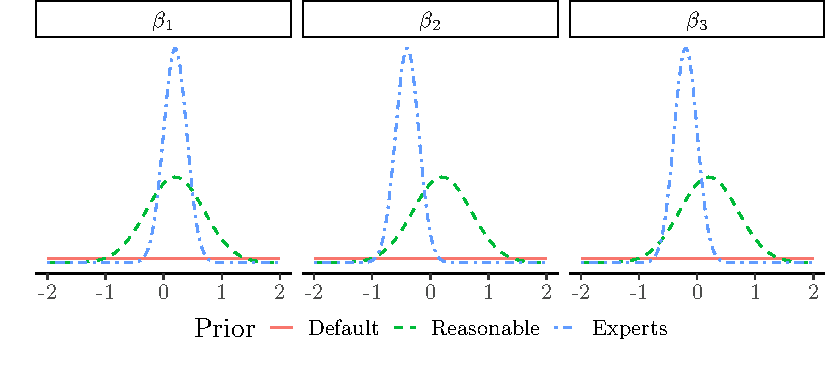
\includegraphics[width = .55\textwidth]{figure/Plot_prior}
	\caption{Prior distribution in the three different settings. Default priors are intended to be non-informative. Reasonable priors  are intended to exclude unplausible values. Experts priors represent experts' judgement.}
	\label{fig:prior}
\end{figure}

 Relative mean bias, relative median bias, mean square error (MSE), coverage and power were considered \cite{smidSemSmallSamples2020}. The relative mean bias (or median bias) evaluates the relative difference between mean estimate ($\bar{\theta}$; or median estimate $\widetilde{\theta}$) across replications and the population value ($\theta$).
% \begin{eqnarray}
% Relative\ mean\ bias = (\bar{\theta}-\theta)/\theta,\\
% Relative\ median\ bias = (\widetilde{\theta}-\theta)/\theta.
% \end{eqnarray}
Relative bias included between -.10 and .10 are considered acceptable \cite{smidSemSmallSamples2020}. MSE takes into account variability as well as bias of the estimates: $MSE = \sigma^2 + (\bar{\theta}- \theta)^2$, where $\sigma$ is the standard deviation of the estimates across replications and $\bar{\theta}$ is the mean. Coverage is the proportion of replications in which the population value is included in the 95\% confidence interval (CI; for the ML estimation) or 95\% highest posterior density interval (HPD; for the Bayesian estimation). Instead, power is the proportion of replications in which the value zero is not included in the 95\% CI or 95\% HPD. Analyses were conducted considering the standardized parameters and for each condition 1000 replications were considered.

\subsection{Results}

The tables with detailed results for each parameter and condition are available at \url{https://osf.io/hwj8d/}. To interpret the results of relative mean and median bias, we considered the distribution of the estimated parameters (see Fig.~\ref{fig:boxplots}).
\begin{figure}[t]
	\sidecaption
	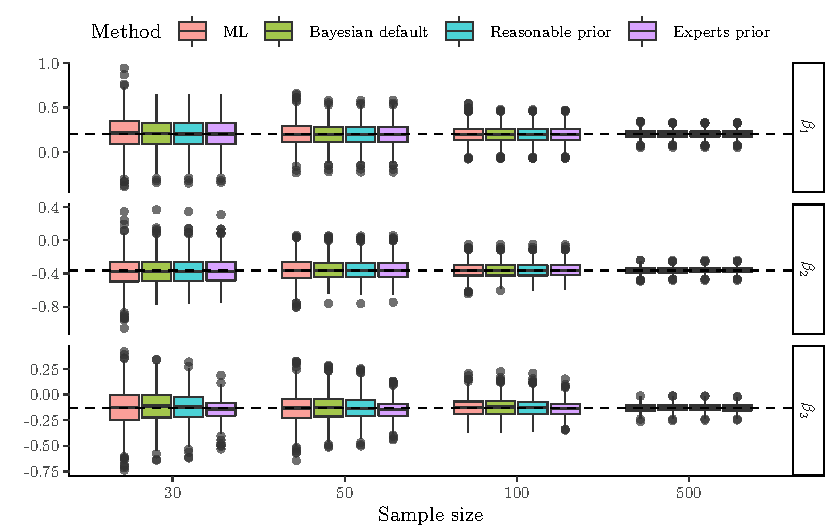
\includegraphics[width = .8\textwidth]{figure/Plot_boxplots}
	\caption{Estimates distribution for each parameter across the different condition. Dashed lines represent the true population values.}
	\label{fig:boxplots}
\end{figure}
Only with very small sample sizes ($n=30$) it is possible to observe some differences between estimation methods: Maximum likelihood approach produces the widest distributions, whereas Bayesian approach with experts prior has narrower distributions. However, differences between methods are noticeable for the parameter $\beta_3$ (i.e., the parameter with the smallest population value) but are less evident for the other parameters and, as the sample size increases, estimation methods perform similar to each other.

Considering the MSE (see Fig.\ref{fig:mse}), we have the same results pattern. Differences between methods are bigger in the case of very small samples ($n=30$), where Bayesian approach with experts prior performs better. However, differences between prior specification are noticeable only for the parameter $\beta_3$.
\begin{figure}[t]
	\sidecaption
	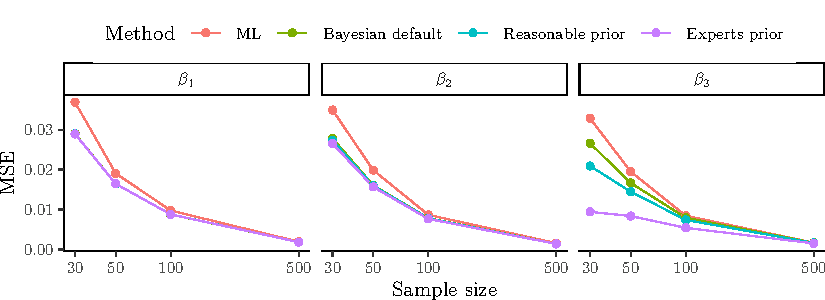
\includegraphics[width = .8\textwidth]{figure/Plot_MSE}
	\caption{Mean Squared Error (MSE) values for each parameter across the different conditions.}
	\label{fig:mse}
\end{figure}

Finally, the result of coverage and power are presented in Fig.~\ref{fig:Plot_coverage_power}.
\begin{figure}[b]
	\sidecaption
	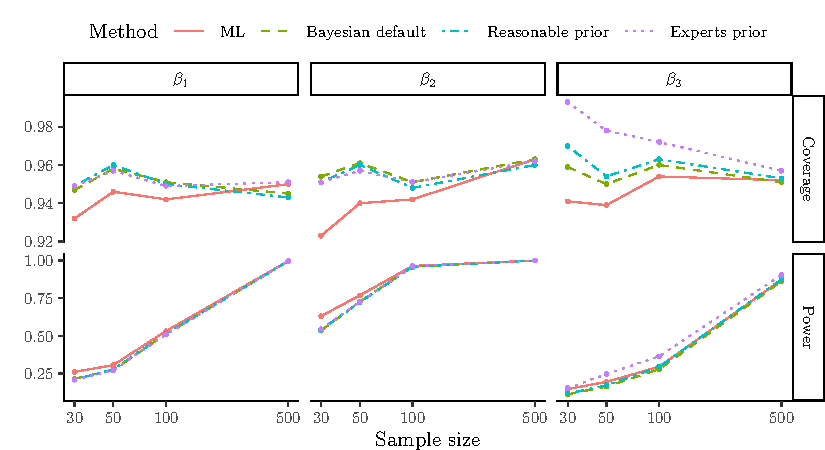
\includegraphics[width = .8\textwidth]{figure/Plot_coverage_power}
	\caption{Coverage and power values for each parameter across the different conditions.}
	\label{fig:Plot_coverage_power}
\end{figure}
Coverage reaches adequate levels in all conditions  with sample size  equal to or greater than 100. With smaller sample sizes, Bayesian approach with experts prior showed excessive coverage in the case of the parameter $\beta_3$. Power is extremely low when sample sizes are small. ML estimation performs slightly better in terms of power across all conditions, except for the  parameter $\beta_3$ where is outperformed by Bayesian approach with experts prior. However, adequate levels of power are reached for all parameters only with large sample sizes ($n = 500$).

\section{Discussion and conclusions}

\label{sec:dicussion}

% In the simulation, we evaluated the different estimation methods in the case of structural equation models with small sample size. Overall, results indicate that informative priors are useful in the case of limited sample sizes and when the true population values are small. When data are limited, the formalization of informative prior according to expert judgement can help in obtaining more accurate results. Parameter estimates were more stable  across replications and extreme values were less likely. When the sample size increases the difference between estimation methods becomes less evident and negligible for sample grater than 100.

In the simulation, we evaluated the different estimation methods in the case of SEMs with small sample size. Overall, results indicate that informative priors are useful in the case of limited sample sizes and when the true population values are small. Parameter estimates were more stable  across replications and extreme values were less likely. When the sample size increases the difference between estimation methods becomes less evident.

However, results are not consistent for all the parameters. In most conditions, Bayesian approach performs better than ML but results are very similar between the different prior specifications. Only in the case of small true population parameter values the Bayesian approach with expert priors performs much better than the other prior specifications.
% Thus, it is necessary to investigate the role of prior definition in models with different structures and levels of complexity, where the dimension of the effects varies.
Future studies should focus on the role of prior definition in SEMs with different levels of complexity (e.g., also taking the measurement part into account) and in which the effect sizes vary on a larger range.
%Another important aspect that future studies should evaluate is the impact of prior knowledge misspecification, in partcular in situations with small sample sizes.

% Another limit in the formalization of priors concerns the definition of inaccurate priors. The more informative the priors are the more accurate results is possible to obtain, as long as priors correctly identify the real population values. However, this is never the case in applied research and inaccurate priors definition could lead to not reliable results. Future studies should evaluate how misspecified priors could influence the results in the case of small sample size.

%In summary, the formalization of informative priors according to expert judgement and relevant knowledge in the field could help in the case of small sample size but further investigation is needed.
% However, we want to highlight that expert knowledge elicitation is not only useful to inform prior distributions but expert knowledge in the field can help also in other aspects of the analysis. Experts can help and inform researchers in the design of the experiments, definition of the models, interpretation of the results and make reasonable and informed choices along all the research process. Thus, the collaboration between different experts is a crucial point that should be encouraged in any applied research field.
Finally, we want to highlight that expert knowledge elicitation is not only useful to inform prior distributions but expert knowledge in the field can help also in other aspects of the analysis. Experts can help and inform researchers in the design of the experiments, definition of the models, interpretation of the results and make reasonable and informed choices along all the research process. Thus, the collaboration between different experts is a crucial point that should be encouraged in any applied research field.

\bibliographystyle{spmpsci.bst}
\bibliography{SIS_2020.bib}


% uncomment the following line to insert reference (dos not work in R-studio, compile with another LaTeX editor)
%%%%%%%%%%%%%%%%%%%%%%%%% referenc.tex %%%%%%%%%%%%%%%%%%%%%%%%%%%%%%
% sample references
% %
% Use this file as a template for your own input.
%
%%%%%%%%%%%%%%%%%%%%%%%% Springer-Verlag %%%%%%%%%%%%%%%%%%%%%%%%%%
%
% BibTeX users please use
% \bibliographystyle{}
% \bibliography{}
%
\biblstarthook{References may be \textit{cited} in the text either by number (preferred) or by author/year.\footnote{Make sure that all references from the list are cited in the text. Those not cited should be moved to a separate \textit{Further Reading} section or chapter.} The reference list should ideally be \textit{sorted} in alphabetical order -- even if reference numbers are used for the their citation in the text. If there are several works by the same author, the following order should be used: 
\begin{enumerate}
\item all works by the author alone, ordered chronologically by year of publication
\item all works by the author with a coauthor, ordered alphabetically by coauthor
\item all works by the author with several coauthors, ordered chronologically by year of publication.
\end{enumerate}
The recommended style for references\footnote{Always use the standard abbreviation of a journal's name according to the ISSN \textit{List of Title Word Abbreviations}.} is depicted in ~\cite{science-contrib, science-online, science-mono, science-journal, science-DOI}.
}

\begin{thebibliography}{99.}%
% and use \bibitem to create references.
%
% Use the following syntax and markup for your references if 
% the subject of your book is from the field 
% "Mathematics, Physics, Statistics, Computer Science"
%
% Contribution 
\bibitem{science-contrib} Broy, M.: Software engineering --- from auxiliary to key technologies. In: Broy, M., Dener, E. (eds.) Software Pioneers, pp. 10-13. Springer, Heidelberg (2002)
%
% Online Document
\bibitem{science-online} Dod, J.: Effective substances. In: The Dictionary of Substances and Their Effects. Royal Society of Chemistry (1999) Available via DIALOG. \\
\url{http://www.rsc.org/dose/title of subordinate document. Cited 15 Jan 1999}
%
% Monograph
\bibitem{science-mono} Geddes, K.O., Czapor, S.R., Labahn, G.: Algorithms for Computer Algebra. Kluwer, Boston (1992) 
%
% Journal article
\bibitem{science-journal} Hamburger, C.: Quasimonotonicity, regularity and duality for nonlinear systems of partial differential equations. Ann. Mat. Pura. Appl. \textbf{169}, 321--354 (1995)
%
% Journal article by DOI
\bibitem{science-DOI} Slifka, M.K., Whitton, J.L.: Clinical implications of dysregulated cytokine production. J. Mol. Med. (2000) doi: 10.1007/s001090000086 
%
\end{thebibliography}

\end{document}
